\documentclass[11pt]{article}
\usepackage{geometry}
\linespread{1.02}
\usepackage{url,epsfig}
\usepackage{relsize}
\usepackage{amsmath}
\usepackage{amssymb}
\usepackage{graphicx}
\graphicspath{{./fig/}}

% For R code snippets
\usepackage{listings}

% Bibliography spacing/indentation
\makeatother\renewcommand{\bibitem}{\vskip 2pt\par\hangindent\parindent\hskip-\parindent}

% Define a bunch of custom math shortcuts for expressions used many times
% throughout the paper
\newcommand{\Rsq}{$r^2\,$}
\newcommand{\boldrho}{\boldsymbol{\rho}}
\newcommand{\boldbeta}{\boldsymbol{\beta}}
\newcommand{\boldtheta}{\boldsymbol{\theta}}
\newcommand{\hatbeta}{\widehat{\boldbeta}}
\newcommand{\hatalpha}{\widehat{\alpha}}
\newcommand{\sigmaEps}{\sigma_{\epsilon}}
\newcommand{\X}{\mathbf{X}}
\newcommand{\y}{\mathbf{y}}
\newcommand{\Q}{\mathbf{Q}}
\newcommand{\R}{\mathbf{R}}
\renewcommand{\u}{\mathbf{u}}
\newcommand{\locRsq}{\ell_{r^2}}
\newcommand{\halfK}{\frac{K}{2}}
\newcommand{\Betadist}[2]{\mathrm{Beta}\left(#1,#2\right)}
\newcommand{\Digamma}[1]{\psi\left(#1\right)}


% Title, authors, date
\title{\bf Regularizing Bayesian linear models with an informative prior on \Rsq
    \vspace{.1in}}
\author{Ben Goodrich\footnote{Columbia University}
    \and Jonah Gabry$^{\ast}$
    \and Andrew Gelman$^{\ast}$
    \and Matthew Stephens\footnote{University of Chicago}
    \vspace{.1in}}
\date{25 February 2016
    \vspace{-.2in}}

% Begin document
\begin{document}
\maketitle
\thispagestyle{empty}

\begin{abstract}
\noindent We derive an approach for expressing prior beliefs about the location
of the \Rsq, the familiar proportion of variance in the outcome variable that is
attributable to the predictors under a linear model. In particular, when there
are many predictors relative to the number of observations we would expect the
joint prior derived here to work better than placing independent, heavy-tailed
priors on the coefficients, which is  standard practice in applied Bayesian data
analysis but neither reflects the beliefs of the researcher nor conveys enough
information to stabilize all the computations.
\end{abstract}


\section{Introduction}

Fully making Bayesian estimation of linear models routine for applied
researchers requires prior distributions that work well for any data generated
according to the assumptions of the likelihood function. Most Bayesian
approaches require the researcher to specify a joint prior distribution for the
regression coefficients (and the intercept and error variance), but most applied
researchers have little inclination to specify all these prior distributions
thoughtfully and take a short-cut by specifying one prior distribution that is
taken to apply to all the regression coefficients as if they were independent of
each other (and the intercept and error variance).

In this paper we derive and demonstrate an approach for expressing  prior
beliefs about the location of the \Rsq, the familiar proportion of variance in
the outcome variable that is attributable to the predictors under a linear
model. Since the \Rsq is a well-understood bounded scalar, it is easy to specify
prior information about it. In particular, when there are many predictors
relative to the number of observations we would expect the joint prior derived
here to work better than placing independent, heavy-tailed priors on the
coefficients, which neither reflects the beliefs of the researcher nor conveys
enough information to stabilize all the computations.


\section{Likelihood}

The likelihood contribution for one observation $y_i$ under a linear model
can be written as the conditionally normal density

$$
f \left(y_i \,|\, \mu_i, \sigmaEps \right) = \frac{1}{\sigmaEps \sqrt{2 \pi}}
\exp{\left\{-\frac{1}{2} \left(\frac{y_i - \mu_i}{\sigmaEps}\right)^2\right\}},
$$
%
where $\mu_i = \alpha + \mathbf{x}_i^\top \boldbeta$ is a linear
predictor and $\sigmaEps$ is the standard deviation of the error in predicting
the outcome. For a sample of size $N$, the likelihood of the entire sample is
the product of the $N$ individual likelihood contributions and it is well known
that the likelihood is maximized when the sum-of-squared residuals is minimized.
This occurs when
%
\begin{align*}
\hatbeta &= \left(\X^\top \X \right)^{-1} \X^\top \y,\\
\hatalpha &= \overline{y} - \overline{\mathbf{x}}^\top \hatbeta,\\
\widehat{\sigma}_{\epsilon}^2 &=
  \frac{1}{N}
  \left(\y - \hatalpha - \X \hatbeta \right)^\top
  \left(\y - \hatalpha - \X \hatbeta \right),
\end{align*}
%
where $\overline{\mathbf{x}}$ is a vector of sample means for the
$K$ predictors, $\X$ is a $N \times K$ matrix of \emph{centered} predictors,
$\y$ is a $N$-vector of outcomes, and $\overline{y}$ is the sample mean of the
outcome.

Taking a QR decomposition of the design matrix, $\X = \Q\R$, where
$\Q^\top \Q = \mathbf{I}$ and $\R$ is upper triangular, we can write the
ordinary least squares (OLS) solution for the regression coefficients as
$$\hatbeta = \left(\X^\top \X \right)^{-1} \X^\top \y = \R^{-1} \Q^\top \y.$$
%
The QR decomposition is often used for improved numerical stability (see the
familiar {\tt lm} function in R), but, as we outline below, it is also useful
for thinking about priors in a Bayesian version of the linear model.


\section{Priors}

The key innovation in this paper is the prior for the parameters in the
QR-reparameterized model, which can be thought of as a prior on the correlations
between the outcome $\y$ and the columns of the orthogonal matrix $\Q$. To
understand this prior, we start with the equations that characterize the maximum
likelihood solutions \emph{before} observing the data $\left(\y, \X\right)$.

Let $\boldtheta = \Q^\top \y$. We can write the $k$-th element of the vector
$\boldtheta$ as
$$\theta_k = \rho_k \sigma_y \sqrt{N - 1},$$
where $\rho_k$ is the correlation between the $k$th column of $\Q$ and the
outcome, $\sigma_y$ is the marginal standard deviation of the outcome, and
$1/\sqrt{N-1}$ is the standard deviation of the $k$ column of $\Q$. Then let
$\boldrho = \sqrt{r^2}\u$, where $\u$ is a unit vector that is
uniformally distributed on the surface of a hypersphere. Consequently,
$\u^\top \u = 1$ implies that the sum of squared correlations is
$\boldrho^\top \boldrho = r^2$, the familiar coefficient of determination for
the linear model.

An uninformative prior on \Rsq would be standard uniform, which is a special
case of a $\Betadist{a}{b}$ distribution with shape parameters $a = b = 1$.
A non-uniform prior on \Rsq is somewhat analogous to ridge
regression, which is popular in data mining and produces better out-of-sample
predictions than least squares because it penalizes $\boldbeta^\top \boldbeta$,
usually after standardizing the predictors. In our case, an informative prior on
\Rsq effectively penalizes $\boldrho^\top \boldrho$, which encourages the
regression coefficients $\boldbeta = \R^{-1} \boldtheta$ to be closer to the
origin.

Consider a correlation matrix among both the outcome and the predictors of
our reparameterized model. Lewandowski, Kurowicka, and Joe (2009) derives a
distribution for a correlation matrix that depends on a single shape parameter
$\eta > 0$ and implies that the conditional variance of one variable given the
remaining $K$ variables is distributed $\Betadist{\eta}{\halfK}$. In our case,
this means that the conditional variance of $\y$ given the predictors,
$1 - r^2$, has a $\Betadist{\eta}{\halfK}$ distribution. From the
reflection symmetry of the Beta distribution, \Rsq is therefore distributed
$\Betadist{\halfK}{\eta}$ and any prior information about the location of \Rsq,
which we will denote $\locRsq$, can be used to choose a value of the
hyperparameter $\eta$.

Four ways of implying a value for $\eta$ via the specification of $\locRsq$ are:

\begin{enumerate}
\item $\locRsq$ is the prior mode on the $\left(0,1\right)$ interval.

This is only valid if $K \geq 2$ since the mode of a $\Betadist{\halfK}{\eta}$
distribution is \newline
$\left(\halfK - 1\right) / \left(\halfK + \eta - 2\right)$
and does not exist if $K < 2$.

\item $\locRsq$ is the prior mean on the $\left(0,1\right)$ interval, where
the mean of a $\Betadist{\halfK}{\eta}$ distribution is
$\left(\halfK\right) / \left(\halfK + \eta\right)$.

\item $\locRsq$ is the prior median on the $\left(0,1\right)$ interval.

The median of a $\Betadist{\halfK}{\eta}$ distribution is not available in
closed form, but if $K > 2$ the median is approximately equal to
$\left(\halfK - \frac{1}{3}\right) / \left(\halfK + \eta - \frac{2}{3}\right)$
(Kerman, 2011). Regardless of whether $K > 2$, we can numerically solve for the
value of $\eta$ that is consistent with a given prior median.

\item $\locRsq$ is some (negative) prior value for
$E\left(\log{r^2}\right) = \Digamma{\halfK} - \Digamma{\halfK + \eta}$,
where $\Digamma{\cdot}$ is the Digamma function. Again, given a prior value for
the left-hand side it is easy to numerically solve for the corresponding value
of $\eta$.
\end{enumerate}
%
Each of these specifications of $\locRsq$ implies a value of the shape parameter
$\eta$, which is the single hyperparameter of the joint prior on the
coefficients. Smaller values for $\locRsq$ will correspond to larger values of
$\eta$, smaller prior correlations among the outcome and predictors, and a prior
density for the regression coefficients more concentrated around zero (see
Figure~\ref{fig:betaplot}).

\begin{figure}
\centering
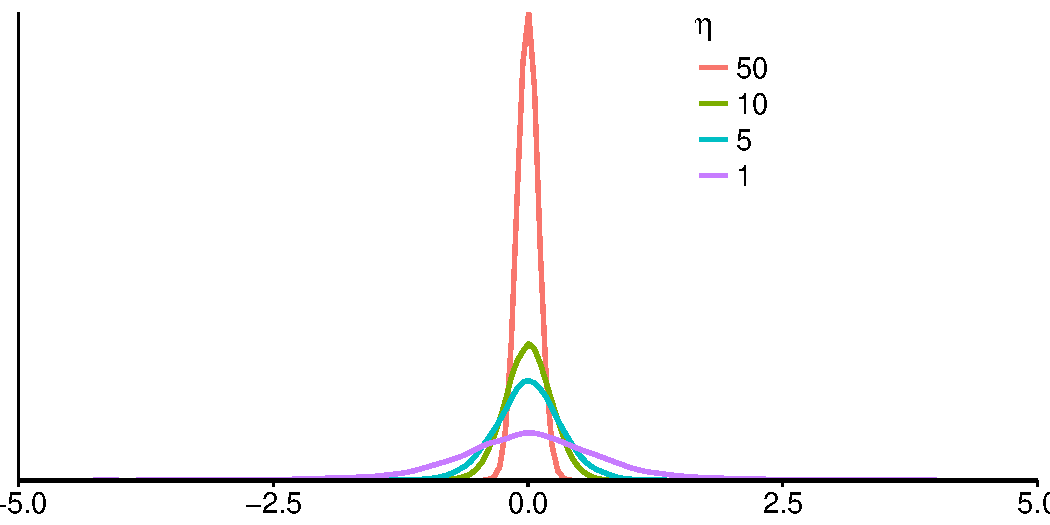
\includegraphics[width=.67\textwidth]{betaplot.pdf}{\vspace{-.5cm}}
\caption{\em Implied marginal prior on standardized regression coefficients
(computed from 100,000 draws) with $K = 10$ and different values for $\eta$. As
$\eta$ increases the prior becomes more concentrated around zero.}
\label{fig:betaplot}
\end{figure}

Next we must specify a prior for $\sigma_y$. We set $\sigma_y = \omega s_y$
where $s_y$ is the sample standard deviation of the outcome and $\omega > 0$ is
an unknown scale parameter to be estimated. The only prior for $\omega$ that
does not contravene Bayes' theorem in this situation is the Jeffreys prior,
$$f_\omega \left(\omega\right) \propto \frac{1}{\omega},$$
which is proportional to a Jeffreys prior on the unknown $\sigma_y$,
$$f_{\sigma_y} \left(\sigma_y\right) \propto \frac{1}{\sigma_y}
= \frac{1}{\omega \widehat{\sigma}_y} \propto \frac{1}{\omega}.$$
This parameterization and prior makes it easy to work with any continuous
outcome variable, no matter what its units of measurement are.

Finally, we need not directly specify a prior for $\sigmaEps$ because our prior
beliefs about $\sigmaEps$ are already implied by our beliefs about $\omega$ and
\Rsq via the relation
$$\sigmaEps = \omega s_y \sqrt{1 - r^2}.$$
Thus, the only remaining distribution to specify is a prior for
$\alpha = \overline{y} - \overline{\mathbf{x}}^\top \R^{-1} \boldtheta$.
As a default, an improper uniform prior is possible as the posterior will still
be proper.


\section{Posterior}

The previous sections imply a posterior distribution for $\omega$, $\alpha$,
$\u$, and \Rsq. After fitting the model, we can recover the parameters
of interest from the primitive parameters as:
%
\begin{align*}
\sigma_y &= \omega s_y \\
\sigmaEps &= \sigma_y \sqrt{1 - r^2} \\
\boldbeta &= \R^{-1} \u \, \sigma_y \sqrt{r^2 \left(N-1\right)}
\end{align*}

When implementing this model, we actually utilize an improper uniform prior on
$\log{\omega}$. Consequently, if $\log{\omega} = 0$, then the marginal standard
deviation of the outcome \emph{implied by the model} is the same as the sample
standard deviation of the outcome. Therefore, if $\log{\omega} > 0$, then the
marginal standard deviation of the outcome implied by the model exceeds the
sample standard deviation, which is to say that the model overfits the data. If
$\log{\omega} < 0$, then the marginal standard deviation of the outcome implied
by the model is less than the sample standard deviation and so the model
underfits the data (or the data-generating process is nonlinear). Given the
regularizing nature of the prior on \Rsq, a minor underfit would be considered
ideal if the goal is to obtain good out-of-sample predictions. If the model
badly underfits or overfits the data, then the model should be reconsidered.


\section{Conclusion}

Priors can be easy or hard for applied researchers to \emph{specify} and easy or
hard for applied researchers to \emph{conceptualize}. Traditional shortcut
priors on regression coefficients are often used because they are both easy to
specify and to conceptualize. The informative prior on \Rsq proposed in this
paper is more difficult to conceptualize, but with the recent release of the
{\tt rstanarm} R package it is equally easy to specify.


\section*{References}

\noindent

\bibitem Gabry, J., and Goodrich, B. (2016). rstanarm: Bayesian Applied
Regression Modeling via Stan. R package version 2.9.0-3.
\url{http://cran.r-project.org/package=rstanarm}

\bibitem Guan, Y., and Stephens, M. (2011). Bayesian variable selection
regression for genome-wide association studies, and other large-scale problems.
\emph{Annals of Applied Statistics}. {\bf 5}(3): 1780--1815.

\bibitem Kerman, J. (2011) A closed-form approximation for the median of the
beta distribution. {\tt arXiv:1111.0433 [math.ST]}.

\bibitem Lewandowski, D., Kurowicka D., and Joe, H. (2009). Generating random
correlation matrices based on vines and extended onion method.
\emph{Journal of Multivariate Analysis}. {\bf 100}(9): 1989--2001.

\bibitem Hothorn, T., and Everitt, B. S. (2015).  HSAUR3: A Handbook of
Statistical Analyses Using R (3rd Edition). R package version 1.0-5.
\url{http://cran.r-project.org/package=HSAUR3}

\bibitem Hothorn, T., and Everitt, B. S. (2014). \emph{A Handbook of
Statistical Analyses Using R}. Chapman \& Hall/CRC, third edition.

\bibitem R Core Team (2015). R: A language and environment for statistical
computing. R Foundation for Statistical Computing, Vienna, Austria.
\url{https://www.R-project.org/}.


\appendix
\clearpage
\section{Example}

\lstset{
    language=R,
    basicstyle=\footnotesize\ttfamily,
    literate={~} {$\sim$}{1}
    }

We will utilize an example from the {\tt HSAUR3} R package, which is used in the
2014 third edition of \emph{A Handbook of Statistical Analyses Using R}.
The model in section 5.3.1 analyzes an experiment where clouds were seeded
with different amounts of silver iodide to see if there was increased rainfall.
This effect could vary according to covariates, which (except for time) are
interacted with the treatment variable. Most people would probably be skeptical
that cloud hacking could explain very much of the variation in rainfall and
thus the prior mode of the \Rsq would probably be fairly small.

The frequentist estimator of this model can be replicated in R by executing

\begin{lstlisting}
> data("clouds", package = "HSAUR3")
> mod <- rainfall ~ seeding * (sne + cloudcover + prewetness + echomotion) + time
> ols <- lm(mod, data = clouds)
\end{lstlisting}

from which we obtain the estimated coefficients

\begin{lstlisting}
> round(coef(ols), digits = 3)
          (Intercept)                      seedingyes
           -0.346                           15.683
          sne                              cloudcover
           0.420                            0.388
          prewetness                       echomotionstationary
           4.108                            3.153
          time                             seedingyes:sne
           -0.045                           -3.197
          seedingyes:cloudcover            seedingyes:prewetness
           -0.486                           -2.557
          seedingyes:echomotionstationary
           -0.562
\end{lstlisting}

Note that we have \emph{not} looked at the estimated \Rsq or $\sigma$ for the
OLS model. We can estimate a Bayesian version of this model using the
{\tt rstanarm} package by prepending {\tt stan\_} to the {\tt lm} call and
specifying a prior mode for \Rsq using the {\tt R2} function:

\begin{lstlisting}
> library("rstanarm")
> post <- stan_lm(mod, data = clouds, prior = R2(location = 0.2, what = "mode"))
\end{lstlisting}

The posterior medians for the coefficients are

\begin{lstlisting}
> round(coef(post), digits = 3)
          (Intercept)                      seedingyes
           2.303                            6.753
          sne                              cloudcover
           0.193                            0.162
          prewetness                       echomotionstationary
           1.751                            1.345
          time                             seedingyes:sne
           -0.019                           -1.407
          seedingyes:cloudcover            seedingyes:prewetness
           -0.204                           -1.068
          seedingyes:echomotionstationary
           -0.264
\end{lstlisting}


The point estimates from the Bayesian model, which are represented by the
posterior medians, appear quite different from the OLS estimates. However, the
{\tt log-fit\_ratio} (i.e. $\log{\omega}$) is quite small

\begin{lstlisting}
> summary(post)["log-fit_ratio", "50%"]
          -0.010
\end{lstlisting}

which indicates that the model only slightly overfits the data when the prior
derived above is utilized. Thus, it would be safe to conclude that the OLS
estimator considerably overfits the data since there are only $24$ observations
with which to estimate $12$ parameters and no prior information is leveraged. In
general, we would expect the prior derived in this paper to be well-suited in
situations like the one above, where there are many predictors relative to the
number of observations.



% End document
\end{document}
